

\chapter{Introduction}



\section{Previous Work}




Much work was done with this configuration by Z. M. Wang in
working towards his Ph.D~\cite{Wang0}.  Wang adapted a type of
photoelectron detector and employed it in various measurements of
atomic rubidium.  This new type of detector allowed for the
measurement of many different atomic parameters in a single
measurement as opposed to previous types of detectors that were
used.

%One of Wang's major accomplishments was in obtaining what he
%calls, "Complete Measurements of Two-Photon Ionization in Atomic
%Rubidium."  Using elliptically polarized light, he excited a
%two-photon ionization of rubidium and collected an image
%representing the resulting photoelectron angular distribution.  By
%fitting the theoretical data to these images, he was able to
%uniquely determine both the ratio of cross sections of the atomic
%$s$- and $d$-waves and the relative phases between the $s$- and
%$d$-waves. This was enough to completely describe the transition.

Wang was also able to measure further properties of atomic
rubidium by running an experiment that employed quantum
interference.  He simultaneously excited both a one- and
two-photon ionization in rubidium using a laser field and its
second harmonic.  This measurement produced a greatly asymmetrical
electron angular distribution due to the quantum interference
effects, and the degree of asymmetry was dependent on the relative
phase of the two laser fields. Again, by fitting the theoretical
data to experimental images, he was able to determine various
parameters of atomic rubidium.  He was able to measure the ratio
of one-photon transition moments and the phase difference between
$p$- and $d$-continuum waves.  These allowed for a complete
description of this transition.

\section{Motivation for Current Work}

While Wang's work was comprehensive in describing the interactions
he was observing, some aspects of the experiment were overlooked
that may affect the measurements that were made.  This applies
specifically to the phase difference between continuum waves found
in the quantum interference experiment.

In order to determine the phase difference between $p$- and
$d$-continuum waves, knowledge of the relative phase of the two
optical fields present is required.  The reason for this will be
demonstrated in section (\ref{theopad}).  The method used to
measure this was to let the fields propagate some distance from
the interaction where a nonlinear crystal converted some of the
fundamental beam into its second harmonic. The second harmonic has
a definite phase relationship to that of the fundamental, so by
measuring the interference between the original second harmonic
field and the newly created second harmonic field, relative phase
at the interaction can be determined.

When the original measurement was done, the phase difference
between the two second harmonic beams was taken to be the same as
the phase difference between the two fields at the interaction.
What was neglected was the fact that there will be some phase
difference that develops between the focused optical fields as
they propagate into the far field region as well as when the
second harmonic is generated.

The present work will be concerned with a calibration of the phase
for the experiment performed by Wang.  The result should be
applicable to many types of coherent control experiments in which
the relative phase between a field and its second harmonic must be
known.


\section{Experimental Overview}
\label{expover}

Since this work represents an extension of previous work performed
by Z. M. Wang, many of the experimental conditions will be the
same as is described in his Ph.D. thesis~\cite{Wang0}.  Much of it
is repeated here for convenience as are the aspects that will be
changed in order to improve his experiment.

The ultimate goal of this experiment is to determine the phase
difference between $p$- and $d$-continuum waves in atomic
rubidium.  This will be done by looking at the quantum
interference between one- and two-photon ionization processes. The
photoelectron angular distribution that results from the process
will be recorded, fitted with theory, and used to determine the
phase difference. A diagram of the experimental setup is shown in
figure (\ref{sysschem}).

\begin{figure}
\includegraphics{optsysschem2}
\caption[Experimental setup]{Experimental setup for the
measurement of the phase difference between $p$- and $d$-continuum
waves in atomic rubidium} \label{sysschem}
\end{figure}

A Q-switched Nd:YAG laser is used as a host to excite a tunable
dye laser that produces a pulsed beam at the fundamental frequency
with a wavelength of 560nm.  This will also be known as the
visible beam.  The beam is amplified and passes through a lens
which will focus it close to where the optic/atom interaction will
take place.  Directly after the lens, the beam enters a
Mach-Zehnder-like setup.  In one branch of the setup, the second
harmonic of the fundamental beam is generated using a nonlinear
$\beta$-Barium Borate (BBO) crystal.  The second harmonic beam has
a wavelength of 280 nm and will also be known as the uv beam.  The
two beams are recombined at the output side of the interferometer.
This type setup allows for very good alignment and overlap of the
two beams which is critical for a strong quantum interference
signal to be detected.

Both the visible and uv beams will be focused to a spot inside a
vacuum system close to the point where they will intersect a beam
of rubidium atoms. The point where they intersect is labelled the
interaction region. Located directly above the interaction is the
Micro Channel Plate (MCP) detector which will collect images of
the photoelectron angular distribution.

After travelling from the interaction region, the two beams will
pass through another BBO crystal (BBO2) which will convert some of
the fundamental beam to its second harmonic.  The original second
harmonic beam will pass through the crystal as well and it will
interfere constructively or destructively with the newly generated
second harmonic. The magnitude of the resulting uv beam exiting
the vacuum system is directly related to the relative phase of the
two beams and will be measured using a photodiode.  This is the
essence of the Phase Detector.

\section{Theoretical Photoelectron Angular Distribution}
\label{theopad}

The measurement of the phase difference between the continuum
waves will be accomplished through measurement of photoelectron
angular distribution (PAD) due to a given laser field.  A general
theory for predicting the electron angular distribution of an atom
was developed by Bebb and Gold~\cite{Bebb}.  The experiment was
performed specifically using the ionization of atomic Rubidium by
a two-color field consisting of a frequency and its second
harmonic with crossed linear polarizations.  The theory of Bebb
and Gold was applied specifically to this condition by Wang and
Elliott~\cite{Wang1} and the resulting angular distribution is
shown in equation (\ref{angdist}).


\begin{equation}
\label{angdist} W (\Theta,\Phi) = \frac{m \left| \vec{k}
\right|}{8\pi^2\hbar} \sum_{i,j=\pm} \left| \frac{eE_o^{2\omega}
exp(i\phi^{2\omega})}{2\hbar}O_{ij}^{(1)} +
\frac{e^2(E_o^{\omega})^2
exp(2i\phi^{\omega})}{4\hbar^2}T_{ij}^{(33)}  \right|^2.
\end{equation}

Where $E_o^{\omega}$ and $E_o^{2\omega}$ refer to the electric
field amplitudes of the fundamental field and its second harmonic,
respectively, and $\phi^{\omega}$ and $\phi^{2\omega}$ refer to
the phase of the fundamental and second harmonic fields,
respectively. The applicable spatial components of the one-photon
transition moment, $O_{ij}^{(1)}$, are given by

\begin{eqnarray}
O_{++}^{(1)} &=& \frac{-4\pi i}{\sqrt{6}} e^{i\xi_p} \left[
-Y_{1,1}R_{3/2} + Y_{1,-1} \left(\frac{R_{3/2} + 2R_{1/2}}{3}
\right) \right] \\
O_{--}^{(1)} &=& \frac{-4\pi i}{\sqrt{6}} e^{i\xi_p} \left[
Y_{1,-1}R_{3/2} - Y_{1,1} \left(\frac{R_{3/2} + 2R_{1/2}}{3}
\right) \right] \\
O_{+-}^{(1)} &=& \frac{-4\pi i}{\sqrt{3}} e^{i\xi_p} Y_{1,0}
\left( \frac{R_{3/2} - R_{1/2}}{3} \right) \\
O_{-+}^{(1)} &=& \frac{4\pi i}{\sqrt{3}} e^{i\xi_p} Y_{1,0} \left(
\frac{R_{3/2} - R_{1/2}}{3} \right).
\end{eqnarray}

The spatial components of the two-photon transition moments,
$T_{ij}^{(33)}$, are given by

\begin{eqnarray}
T_{++}^{(33)} &=& \frac{1}{3}e^{i \xi_s}Y_{0,0}S_{\bar{s}} -
\frac{2}{3\sqrt{5}}e^{\xi_d}Y_{2,0}S_{\bar{d}} \\
T_{--}^{(33)} &=& \frac{1}{3}e^{i \xi_s}Y_{0,0}S_{\bar{s}} -
\frac{2}{3\sqrt{5}}e^{\xi_d}Y_{2,0}S_{\bar{d}} \\
T_{+-}^{(33)}&=&
\sqrt{\frac{2}{15}} e^{i\xi_d} Y_{2,1} S_{\Delta d} \\
T_{-+}^{(33)} &=& \sqrt{\frac{2}{15}} e^{i\xi_d} Y_{2,-1}
S_{\Delta d}.
\end{eqnarray}

In the above equations, $Y_{l,m}$ is the spherical harmonic
function, $\xi_{s,p,d}$ is the phase of the $s$, $p$, or $d$
partial wave, and $R_{1/2, 3/2}$ is the single-photon transition
moment. The following substitutions were made.

\begin{equation}
S_{\bar{s}} = \frac{S_1+2S_2}{3} ; S_{\bar{d}} =
\frac{5S_3+S_4+9S_5}{15} ; S_{\Delta d} = \frac{5S_3+S_4-6S_6}{15}
\end{equation}

The terms $S_{1-5}$ refer to the two-photon radial transition
matrix elements.  If the above substitutions are made into
equation (\ref{angdist}), it can be simplified into the following
form.

\begin{eqnarray*}
\label{angdistsimp}
& & W(\Theta,\Phi) \propto\\
& & \left| M_R e^{i\phi_{2 \omega} - 2i\phi_{\omega}}
e^{i(\xi_p-\xi_d)} \frac {-4\pi i}{\sqrt{6}} \left[ -Y_{1,1} +
Y_{1,-1}\frac{1+2 \frac{R_{1/2}}{R_{3/2}}}{3} \right] +
 \left[ \frac{1}{3} e^{i(\xi_s - \xi_d)} Y_{0,0} \frac{S_{\bar{s}}}{S_{\bar{d}}} -\frac{2}{3\sqrt{5}}Y_{2,0} \right] \right|^2  \\
& + & \left|M_R e^{i\phi_{2 \omega} - 2i\phi_{\omega}}
e^{i(\xi_p-\xi_d)} \frac {-4\pi i}{\sqrt{3}} Y_{1,0}\frac{1 -
\frac{R_{1/2}}{R_{3/2}}}{3} +
 \sqrt{\frac{2}{15}} Y_{2,1} \frac{S_{\Delta d}}{S_{\bar{d}}} \right|^2  \\
&  + & \left| M_R e^{i\phi_{2 \omega} - 2i\phi_{\omega}}
e^{i(\xi_p-\xi_d)} \frac {4\pi i}{\sqrt{3}} Y_{1,0} \frac{1 -
\frac{R_{1/2}}{R_{3/2}}}{3} +
 \sqrt{\frac{2}{15}} Y_{2,-1} \frac{S_{\Delta d}}{S_{\bar{d}}} \right|^2 \\
& + & \left| M_R e^{i\phi_{2 \omega} - 2i\phi_{\omega}}
e^{i(\xi_p-\xi_d)} \frac {-4\pi i}{\sqrt{6}} \left[ Y_{1,-1} -
Y_{1,1}\frac{1+2 \frac{R_{1/2}}{R_{3/2}}}{3} \right] +
 \left[ \frac{1}{3} e^{i(\xi_s - \xi_d)} Y_{0,0} \frac{S_{\bar{s}}}{S_{\bar{d}}} -\frac{2}{3\sqrt{5}}Y_{2,0} \right]
 \right|^2,
\end{eqnarray*}where $M_R$ is the relative magnitude of the one-photon process to
that of the two-photon process.  It can clearly be seen from
equation (\ref{angdistsimp}) that in order to determine the
continuum phase difference, $\xi_p-\xi_d$, from a fit to this
equation, it is necessary to know the optical phase difference,
$\phi_{2 \omega} - 2\phi_{\omega}$.
 Many of the quantities of equation (\ref{angdistsimp}) have been
previously determined by Wang and Elliott~\cite{Wang1, Wang2}.
These quantities are shown in table (\ref{angdistvalues}).

\begin{table}[h]
\caption[Known Quantities in Angular Distribution Function]{Values
of known quantities used in equation (\ref{angdistsimp})}
\label{angdistvalues}
  \centering
\begin{tabular}{|c|r|}
\hline
Quantity&Value\\
\hline
$\frac{R_{1/2}}{R_{3/2}}$&1.96\\
$\frac{S_{\bar{s}}}{S_{\bar{d}}}$&-0.42\\
$\frac{S_{\Delta d}}{S_{\bar{d}}}$&-0.36\\
$\xi_s-\xi_d$&2.08\\
\hline
\end{tabular}

\end{table}

Using equation (\ref{angdistsimp}) and the properties of the
detector system used by Wang~\cite{Wang0} it is possible to
develop expected angular distributions and the corresponding
images that will be detected.  Some example calculated images are
shown in figure (\ref{extheo}).

\begin{figure}
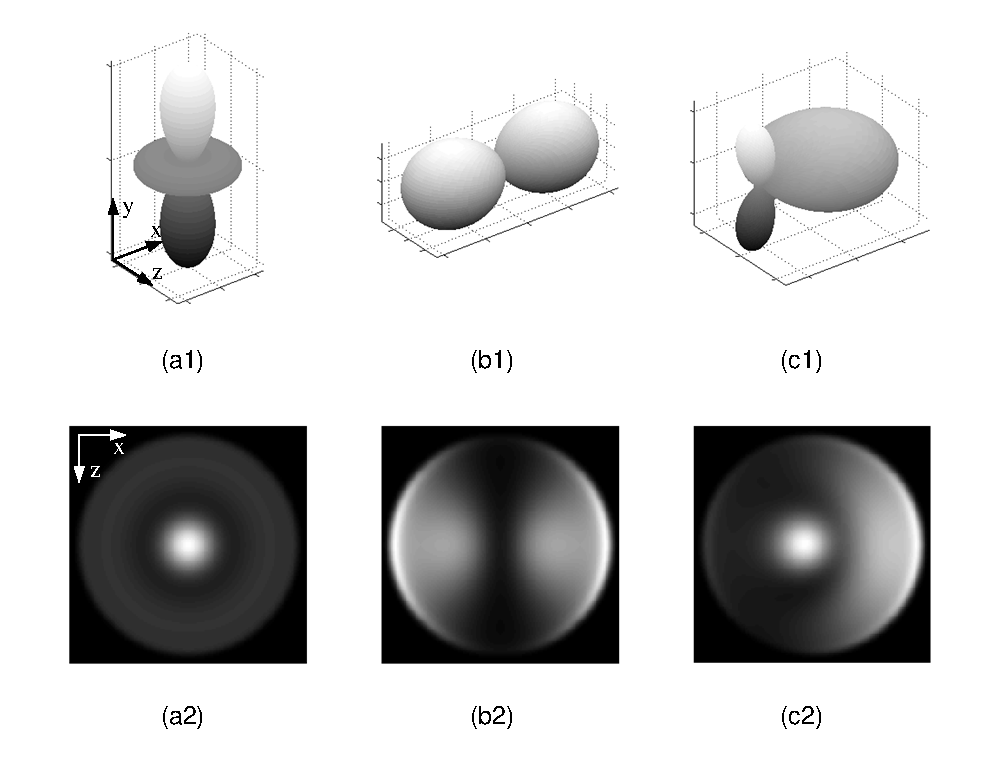
\includegraphics{extheo}
\caption[Example theoretical angular distributions and
images]{Examples of various angular distributions, (x1), and their
corresponding images, (x2) on the detector system.  Images (a1,2)
represent the result of excitation due to a field of wavelength
560 nm that is vertically polarized.  Images (b1,2) are due to a
horizontally polarized field at 280 nm.  Images (c1,2) represent a
result having both fields present.} \label{extheo}
\end{figure}
